% accentcolor - https://www.tu-darmstadt.de/media/medien_stabsstelle_km/services/medien_cd/das_bild_der_tu_darmstadt.pdf (pages 17-18)
% amsmath	- formatting math stuff	(ftp://ftp.ams.org/pub/tex/doc/amsmath/amsldoc.pdf)
% enumitem	- formatting enumerates	(http://ftp.uni-erlangen.de/ctan/macros/latex/contrib/enumitem/enumitem.pdf)
% graphicx	- images				(http://ctan.space-pro.be/tex-archive/macros/latex/required/graphics/grfguide.pdf)
% lipsum	- lorem ipsum			(ftp://ftp.fu-berlin.de/tex/CTAN/macros/latex/contrib/lipsum/lipsum.pdf)
% listings	- source code			(http://texdoc.net/texmf-dist/doc/latex/listings/listings.pdf)
% mathtools	- amsmath extension		(ftp://ftp.fu-berlin.de/tex/CTAN/macros/latex/contrib/mathtools/mathtools.pdf)
% parskip	- splittitle 
\documentclass[11pt, accentcolor=tud1c]{tudreport}	
\usepackage[english]{babel}
\usepackage[utf8]{inputenc}
\usepackage{amsmath, enumitem, graphicx, hyperref, lipsum, listings, mathtools, parcolumns, pdfpages, subcaption, parskip}
\raggedbottom

% https://scm.informatik.tu-darmstadt.de/news/129-technical-documentation-sample


% Specifying new commands
\newcommand{\titlerow}[2]{
    \begin{parcolumns}[colwidths={1=.15\linewidth}]{2}
        \colchunk[1]{#1:}
        \colchunk[2]{#2}
    \end{parcolumns}
    \vspace{0.2cm}
}

% configuring title
\title{Internet-Praktikum: Telekooperation}
\setinstitutionlogo{./res/logo.pdf}

\subtitle{
	\titlerow{Project}{Sechzehn}
	\titlerow{Team Bravo}{Alexander Geiß {\small(alexanderhelmut.geiss@stud.tu-darmstadt.de)}, \\ 
	                      Lukas Klein {\small(lukas.klein@stud.tu-darmstadt.de)},  \\ 
	                      Martin Lichtblau {\small(martin.lichtblau@stud.tu-darmstadt.de)}, \\ 
	                      Johannes Semsch {\small(johannesmaximilianchristian.semsch@stud.tu-darmstadt.de)}, \\ 
	                      Tim Walter {\small(tim.walter.10@stud.tu-darmstadt.de)}}
}



% document 
\begin{document}

\maketitle
\tableofcontents

\chapter{Motivation}\label{ch:motivation}
% ! max. 1 page !
With the backing of its helpful and positive community, ``Sechzehn'' guides you through venues all around the world. 
Places like restaurants and museums are collectively rated. Each and every user of ``Sechzehn'' has the ability to share his personal experiences with the whole community. 
Our rating not only includes a textual rating system, it also allows the user to upload photos taken at this place. Furthermore we also offer a short like and dislike rating. \\\\
``Sechzehn'' also has a social component. You see other members of our community on a map. This map combined with our real-time chat paves the way to quickly establish new and long-lasting friendships.
Our real-time chats focuses on the most important features a messenger should have. This includes read receipts and the transmission of emojis. We do not distract you with features no one needs like photo filters and drawing capabilities in the chat.
To satisfy more privacy-aware users who might not be happy with frequent position updates, we also provide an incognito mode. If the user enters it, he is not displayed on the map of other users. 
This feature makes it possible to use our app if the user is somewhere where he is not expected to be. \\\\
An intuitive and enjoyable user experience is important for us. That's why we designed our app following the material design guidelines.

% datenschutz
% pure material design 
% Also maintaining friednships is easier than ever since friends are specially highlighted on the map

% Soziale App; zeigt nicht nur Venues
% Man sieht wenn Freunde an einem Ort sind und kann aus Gruppen von vielen Menschen auf Events schliessen
% Nachrichtenaustausch moeglich
%%


\chapter{Overview}\label{ch:overview}
% ! image demanded !
In this section we present the architecture we used and thereby how our components interact with each other. We then briefly describe which technologies we chose, and why we chose them.
\section{Architecture}\label{sec:architecture}
% components and their interaction
\subsection{Interaction of Components}
\begin{figure}[ht]
	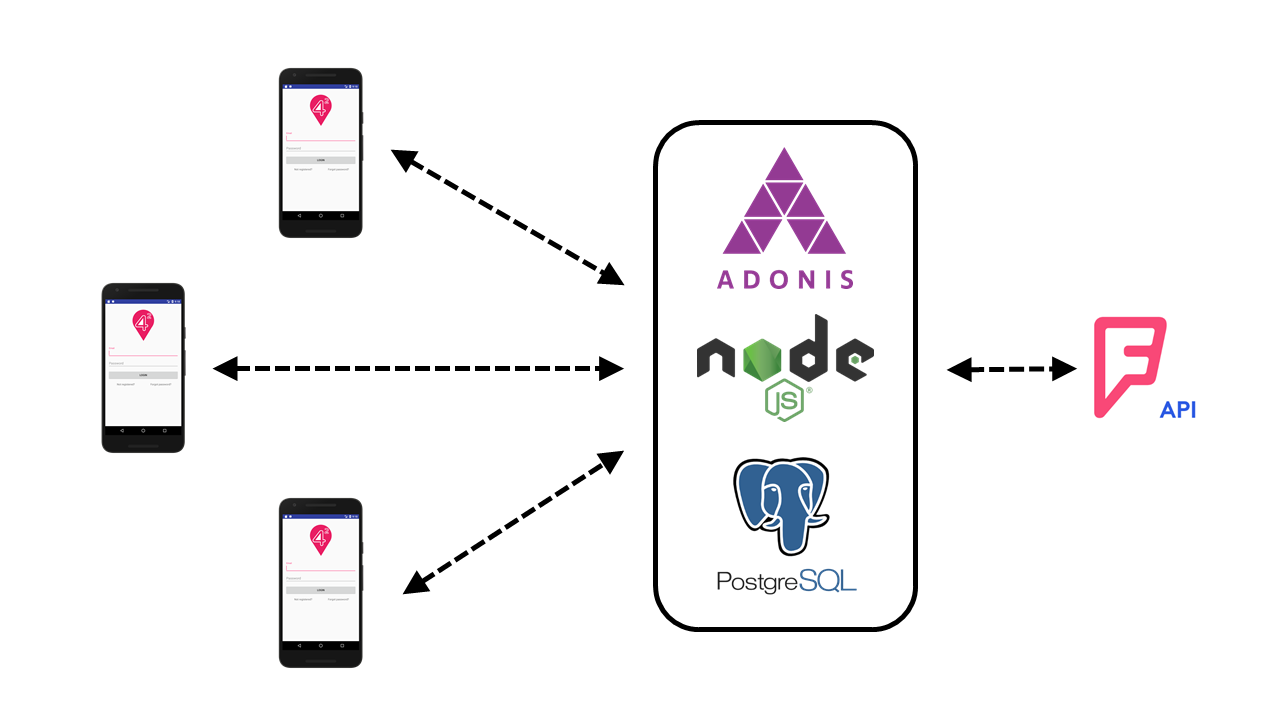
\includegraphics[width=\textwidth]{./res/architecture.png}
	\caption{Architecture}
	\label{fig:architecture}
\end{figure}
The communication between the clients and our server is illustrated in \autoref{fig:architecture}.
For their communication with our server, the clients access the RESTful endpoints or use WebSocket connections. The latter one is necessary to provide our real-time chat. Since we do not have a huge community that backs our app, we need to retrieve the data from other sources. Our server therefore connects to the Foursquare API and fetches the venues, venue details and photos dynamically.
\clearpage
\subsection{Server API Documentation}
To connect app and server, the app developers need the knowledge of endpoints, query parameters and the data structures of requests and responses. To prevent that they need to look through the server's code, an extensive documentation is provided using Apiary \cite{apiary}. An impression is given in \autoref{fig:apiary}.

\begin{figure}[ht]
	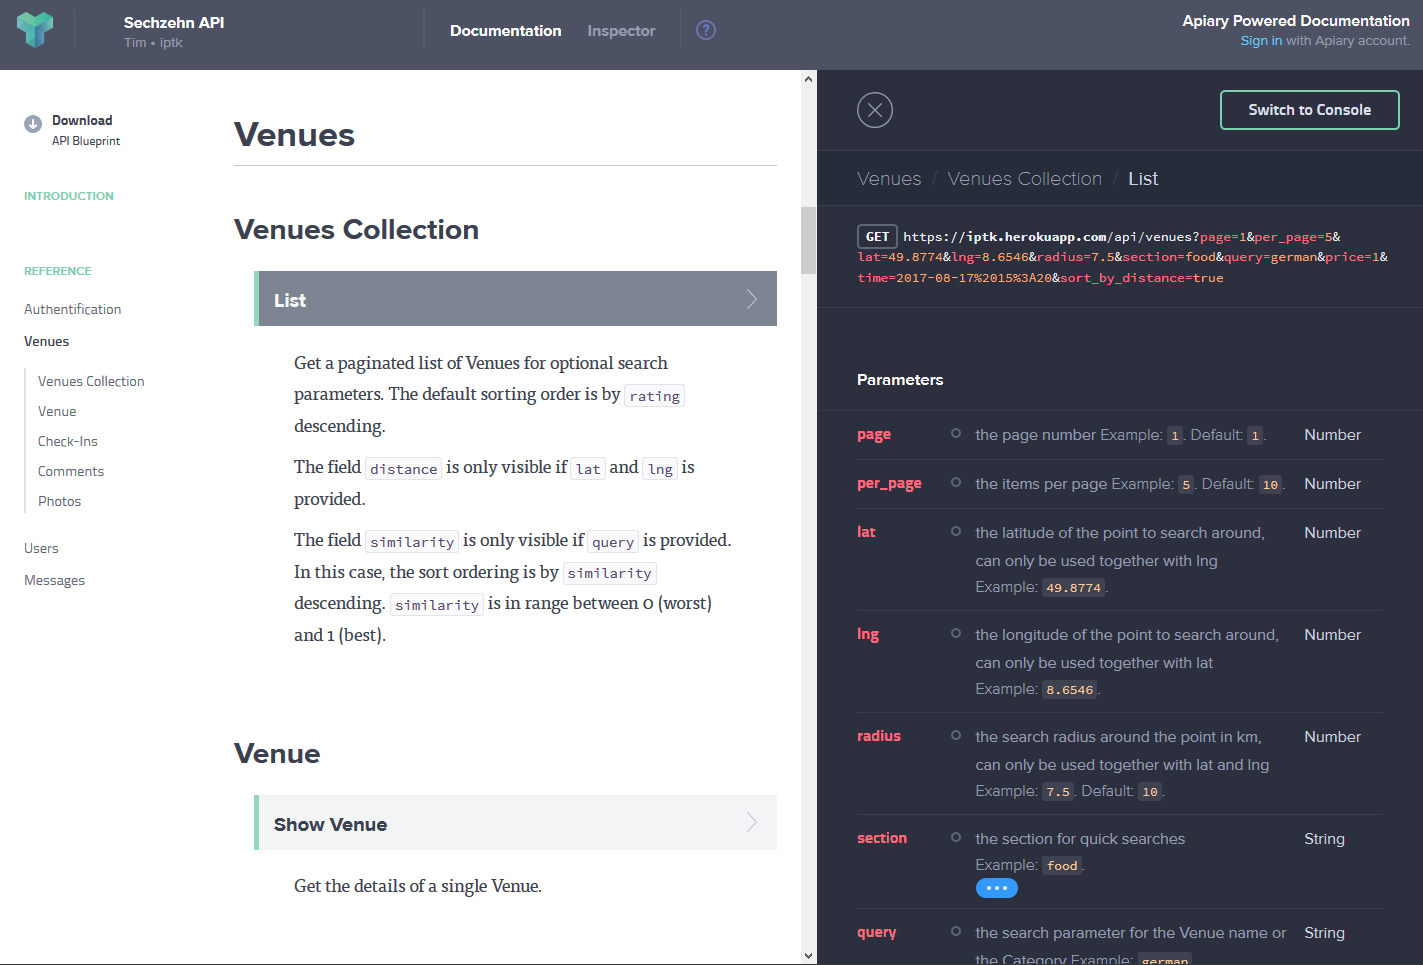
\includegraphics[width=\textwidth]{./res/apiary.png}
	\caption{Screenshot of the Apiary Documentation}
	\label{fig:apiary}
\end{figure}

\clearpage
\subsection{Database}
\begin{figure}[ht]
	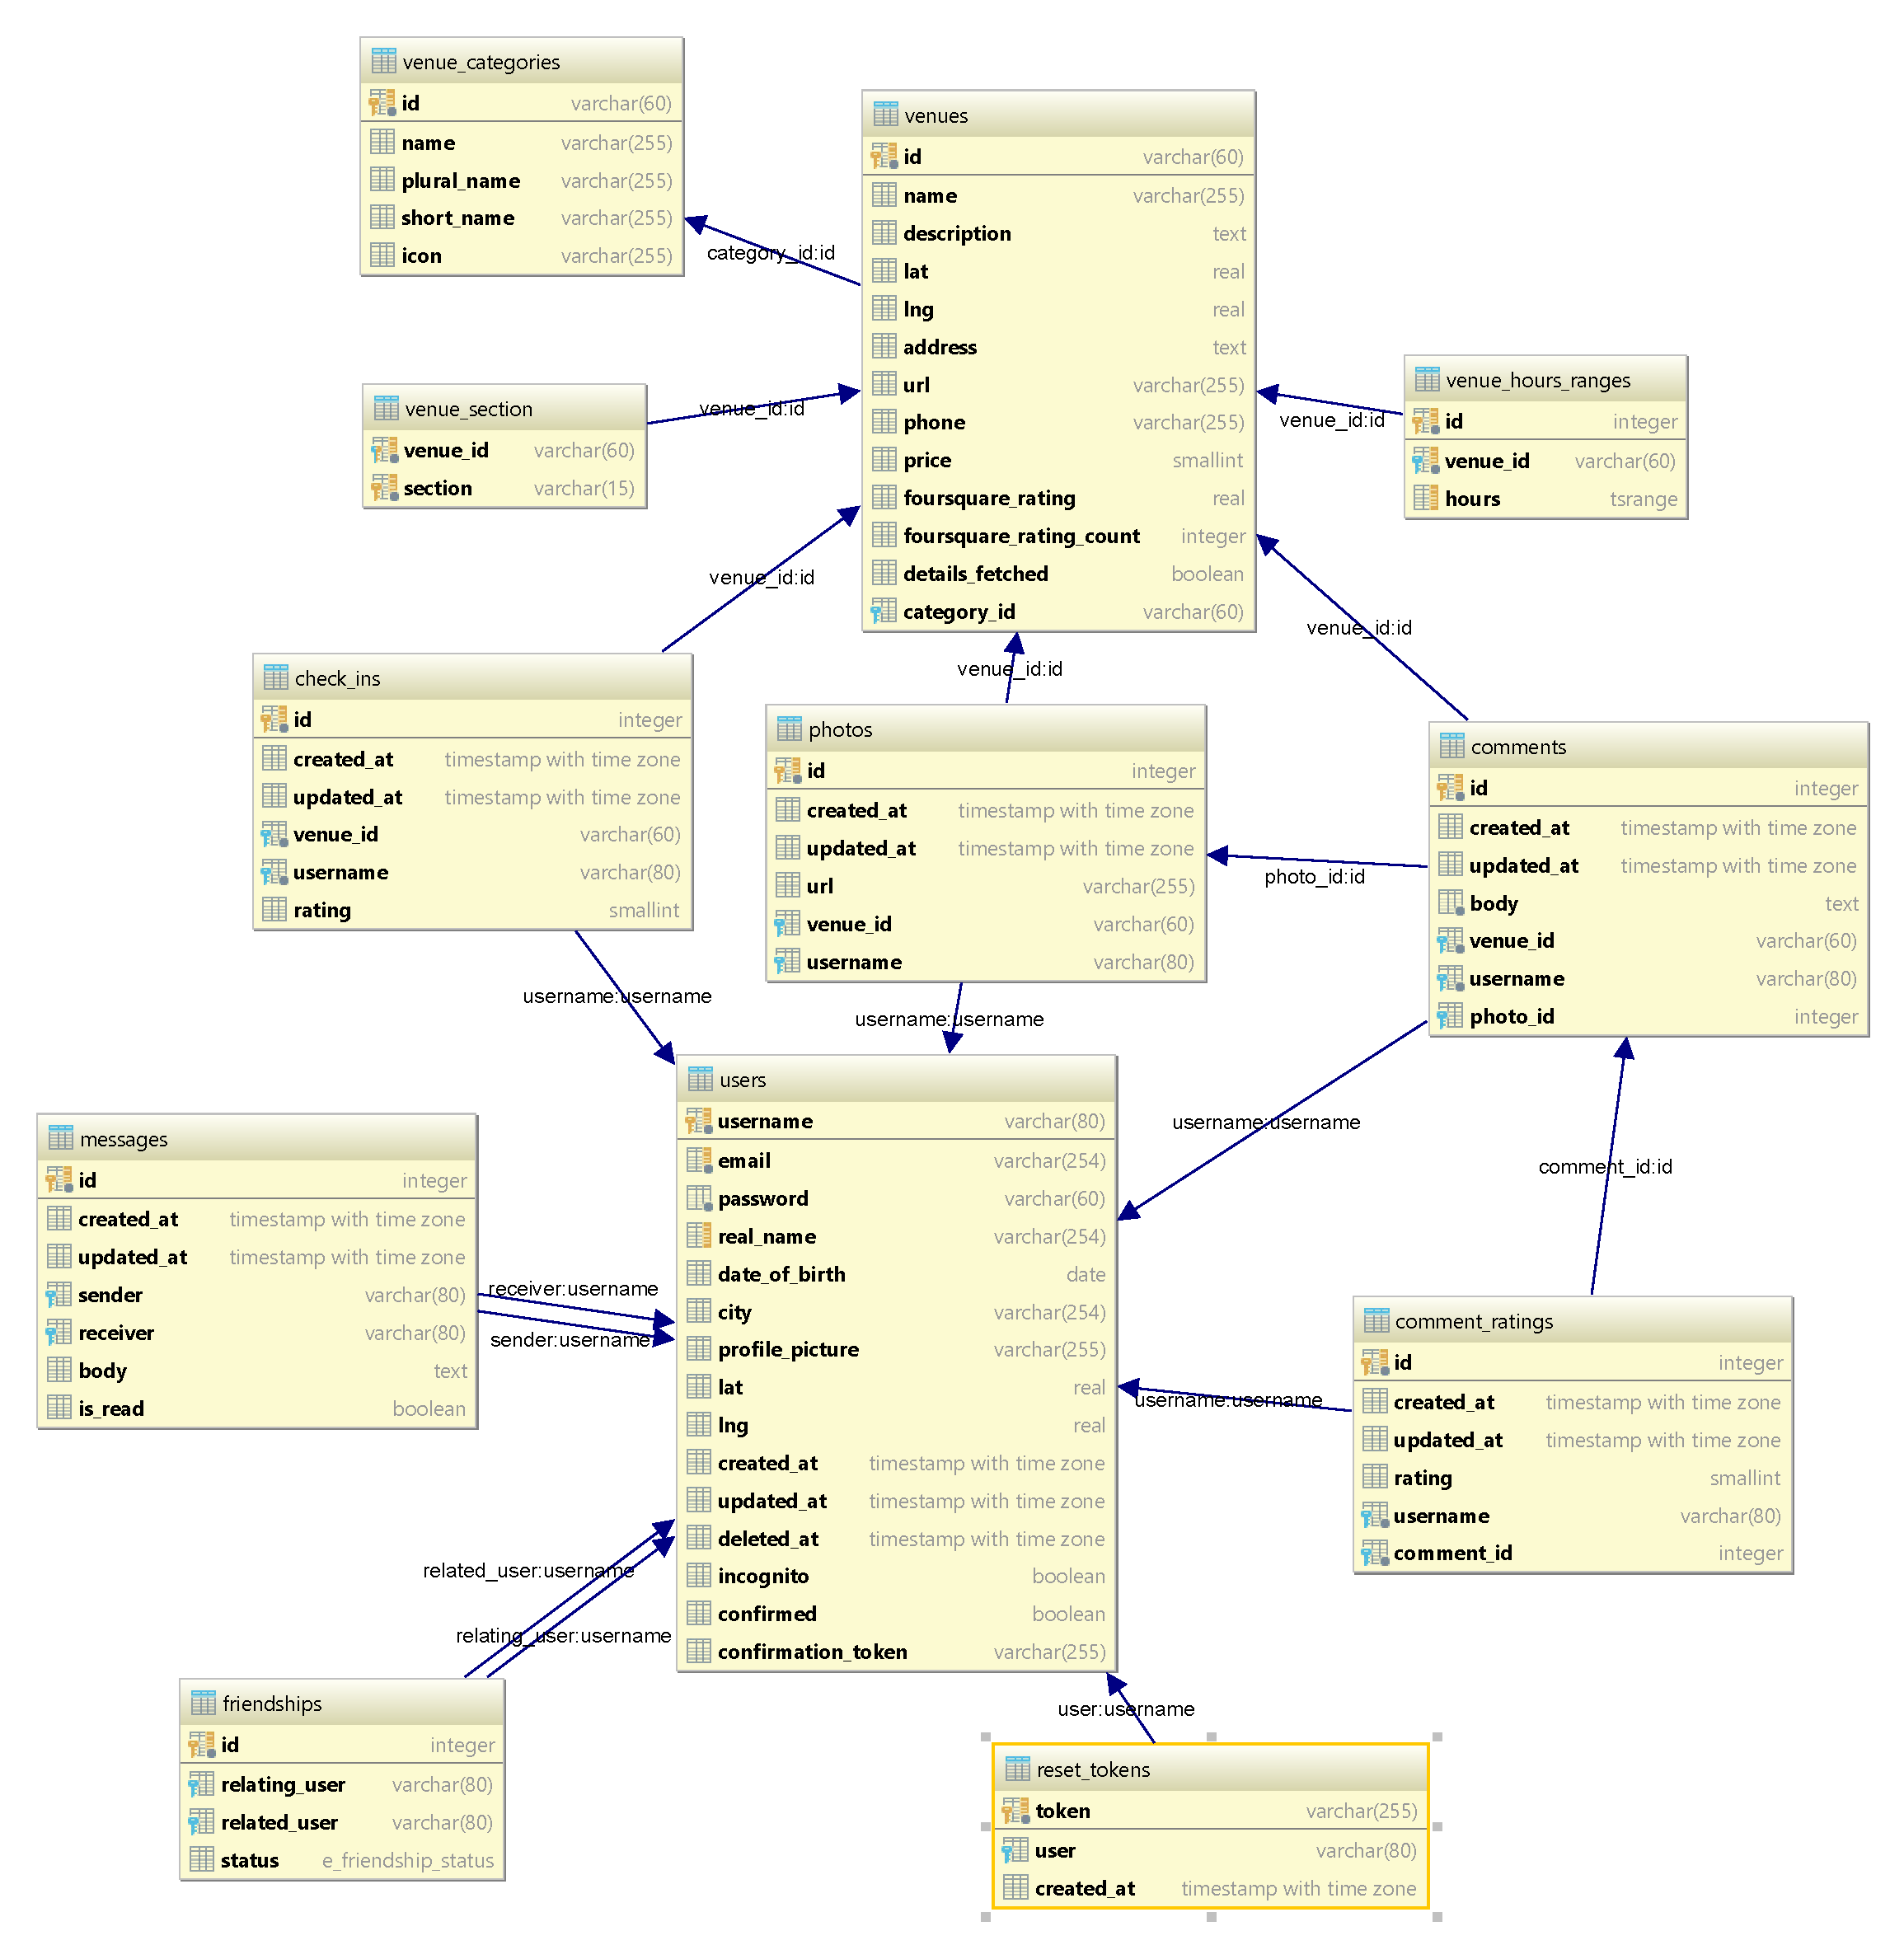
\includegraphics[width=\textwidth]{./res/sechzehn-erm.pdf}
	\caption{Database scheme}
	\label{fig:database_scheme}
\end{figure}

\section{Server}\label{sec:server}
To host our server we use the Heroku Cloud Application Platform \cite{heroku}. Heroku provides us a PostgreSQL \cite{postgresql} database service and an Node.js execution environment. Furthermore it offers access to Cloudinary \cite{cloudinary} image storage service that can be used as plugin within heroku. Heroku offers a free plan ``hobby-dev'' that we use.

\subsection{Node.js}

Node.js \cite{Node.js} is a cross-platform environment that allows building web servers with JavaScript.
This is contrary to the usual applications that are written in JavaScript since it was firstly designed to be a client-side scripting language for browsers. Node.js in its current version also supports asynchronous execution and concepts like generator functions. This allows easy-readable code on a high abstraction level with high-order functions and a good handling of asynchronous operations.

\subsection{AdonisJs}\label{sec:adonisjs}
AdonisJs \cite{adonisjs} is a MVC framework for Node.js web applications. It offers a further layer of abstraction and handles HTTP routing, requests and responses, content negotiation and an object-relational mapping to persist and fetch models from the database. In addition, it provides APIs for user input validation and sanitization, mail sending with templates, omitting fields from JSON output and authentication middleware. Due to this abstraction, it is not necessary to deal with unpretentious programming work that has been done multiple times before and is always the same for web application (e.g. routing, templating, authentication). 

\subsection{PostgreSQL}
PostgreSQL \cite{postgresql} is a powerful open-source relational database management system. It provides the ability to add useful extensions, new data types and functions. We use extensions to determine if a venue or another user is near to the user's current position and to compute a similarity metric on two strings. The latter is the basis of the venue and user search. PostgreSQL offers data types for time ranges that allow to search for open venues. In this context, a custom function is used to convert opening hours into an unambiguous database representation that prevent overlaps. Fortunately, heroku provides a PostgreSQL plugin.

\subsection{JSON Web Tokens}\label{sec:json_web_tokens}
The authentication in our project is done with JSON Web Tokens (JWTs) \cite{jwt}. Given a secure connection, JWTs offer a secure, stateless authentication methods that renders sessions and cookies unnecessary.

\section{Client}\label{sec:client}
\subsection{Android Data Binding}
Android Data Binding \cite{databinding} enables us to write declarative layouts. Those can be easily adapted with new data in various forms by just passing a data object. Therefore it minimizes the amount of glue code needed. Furthermore it implements a kind of view holder pattern, so it is not necessary to use \texttt{findViewById} since all views are available through the binding object.
\subsection{Retrofit}
In our app HTTP requests are done with Retrofit\cite{retrofit}. Retrofit is a type-safe client for Android that helps the developer to retrieve and upload structured data like JSON via a REST based web service. Retrofit itself is based on the OkHttp Library. We chose to use Retrofit because it is a state-of-the-art technology that is also recommended by the Google Guidelines.
\subsection{GSON}
GSON\cite{gson} is a Java library that offers a simple way to serialize and deserialize JSON Objects to Java Objects and the other way around. One of the reason why we chose it, that it does not require additional class annotations like alternative libraries do. GSON is well documented and developed (and recommended) by Google.
\subsection{ChatKit}
ChatKit for Android \cite{chatkit} is a library that is designed to simplify the UI development of WebSocket based chats in Android. It offers predefined components like Dialog Lists, Message Lists, and Message Input. Furthermore it provides state-of-the-art messaging features like read receipts without too much additional effort.


\chapter{App and Feature Explanation}\label{ch:app_and_feature_explanation}

\section{System Requirements}\label{sec:system_requirements}
%minSDK 23 %% compileSDK 25 ??? %% Permissions and justification why they are necessary
To run the app with all features Android Marshmallow (API 23) is needed. 
In this section we briefly describe which permissions are requested by the app and why they are necessary.
\begin{enumerate}
\item Permission to take pictures and videos: This permission allows us to take pictures and add them to venues.
\item Permission to get access to pictures, media, and files on the device: Normally users use profile pictures for more than one app, what makes it necessary to load those pictures from the gallery. This permission is further needed to store the users login credentials on the phone.
\item Permission to have access to the location of the device: The whole concept of the app is based on the users location. The location is necessary to see users and venues in the surroundings. With an incognito switch however, the user can hide his account from the map.
\end{enumerate}

\section{Get Started}

To install the app the user has to put the APK file from our git repo on his phone. The next step is installing the APK by tapping on it in the file explorer of your choice. If the users phone has not the permission to install apps from third parties, he has to allow the phone to install apps from third parties. This is described by the following steps (some phones will directly lead the user to step 3):
\begin{enumerate}
\item go to ``Settings'',
\item choose ``Security'',
\item scroll to ``Unknown sources'' and
\item allow the installation from unknown sources.
\end{enumerate} 
If the users phone is allowed to install apps from third parties, the phone asks the user to install the app. To do so he has to tap on install. The app is now installed successfully.

\section{Features}\label{sec:features}
We only list the bonus features because the mandatory features have to be fulfilled.

\begin{enumerate}
\item Account verification with an email: \\
After registering the email has to be verified first. Without this verification, the user cannot use the app.
\item Open the links from the emails: \\
After resetting your password or registering a new account the user receives an email containing a link. Our app is able to handle this link on click. This means that no verification code must be entered and no external browser is necessary to do this.
\item Resource-efficient location updating: \\
To treat the users battery with care, we use the Google Location Services. If another app on the system requests the location via those location services, we use the new location if it is more accurate. If there hasn't been a request for more than two minutes our app self starts a request to the location services. More inaccurate locations are used after ten minutes without an more accurate position. Furthermore we only push our new location to the ``Sechzehn'' servers, when the user moved more than 100 meters. 
\item Incognito Mode: \\
Within his settings the user can disable that other users of ``Sechzehn'' can see his position. This feature allows privacy without logging out.
\item Live Chats: \\
Our app not only gives you the opportunity to see friends on a map, you can also contact them via live chats. Those live chats also support read receipts.
\item Venue Filters: \\
The venue search offers filtering for opening hours and price category.
\item Push Notifications: \\
The user receives push notifications if a new message is sent to him.
\item Web Interface: \\
We also provide a web interface to confirm email addresses and set new passwords.
\item Live Updates: \\
The location is updated every 100m to provide a near to real-time feeling.
\item Encryption: \\
We use TLS as transport encryption to prevent eavesdropping.
\item Venue Marker Coloured by Rating:\\
Our venue markers are coloured by the rating of the venue. Where green means a higher rating and red a lower rating. The colours of other ratings are interpolated between these colours.
\end{enumerate}

\section{App Flow}
% system requirements, get started, functionalities, features, app flow, ...
%%%LOGIN SCREEN%%%
\begin{figure}[h]
\centering
\begin{minipage}{.3\textwidth}
  \centering
  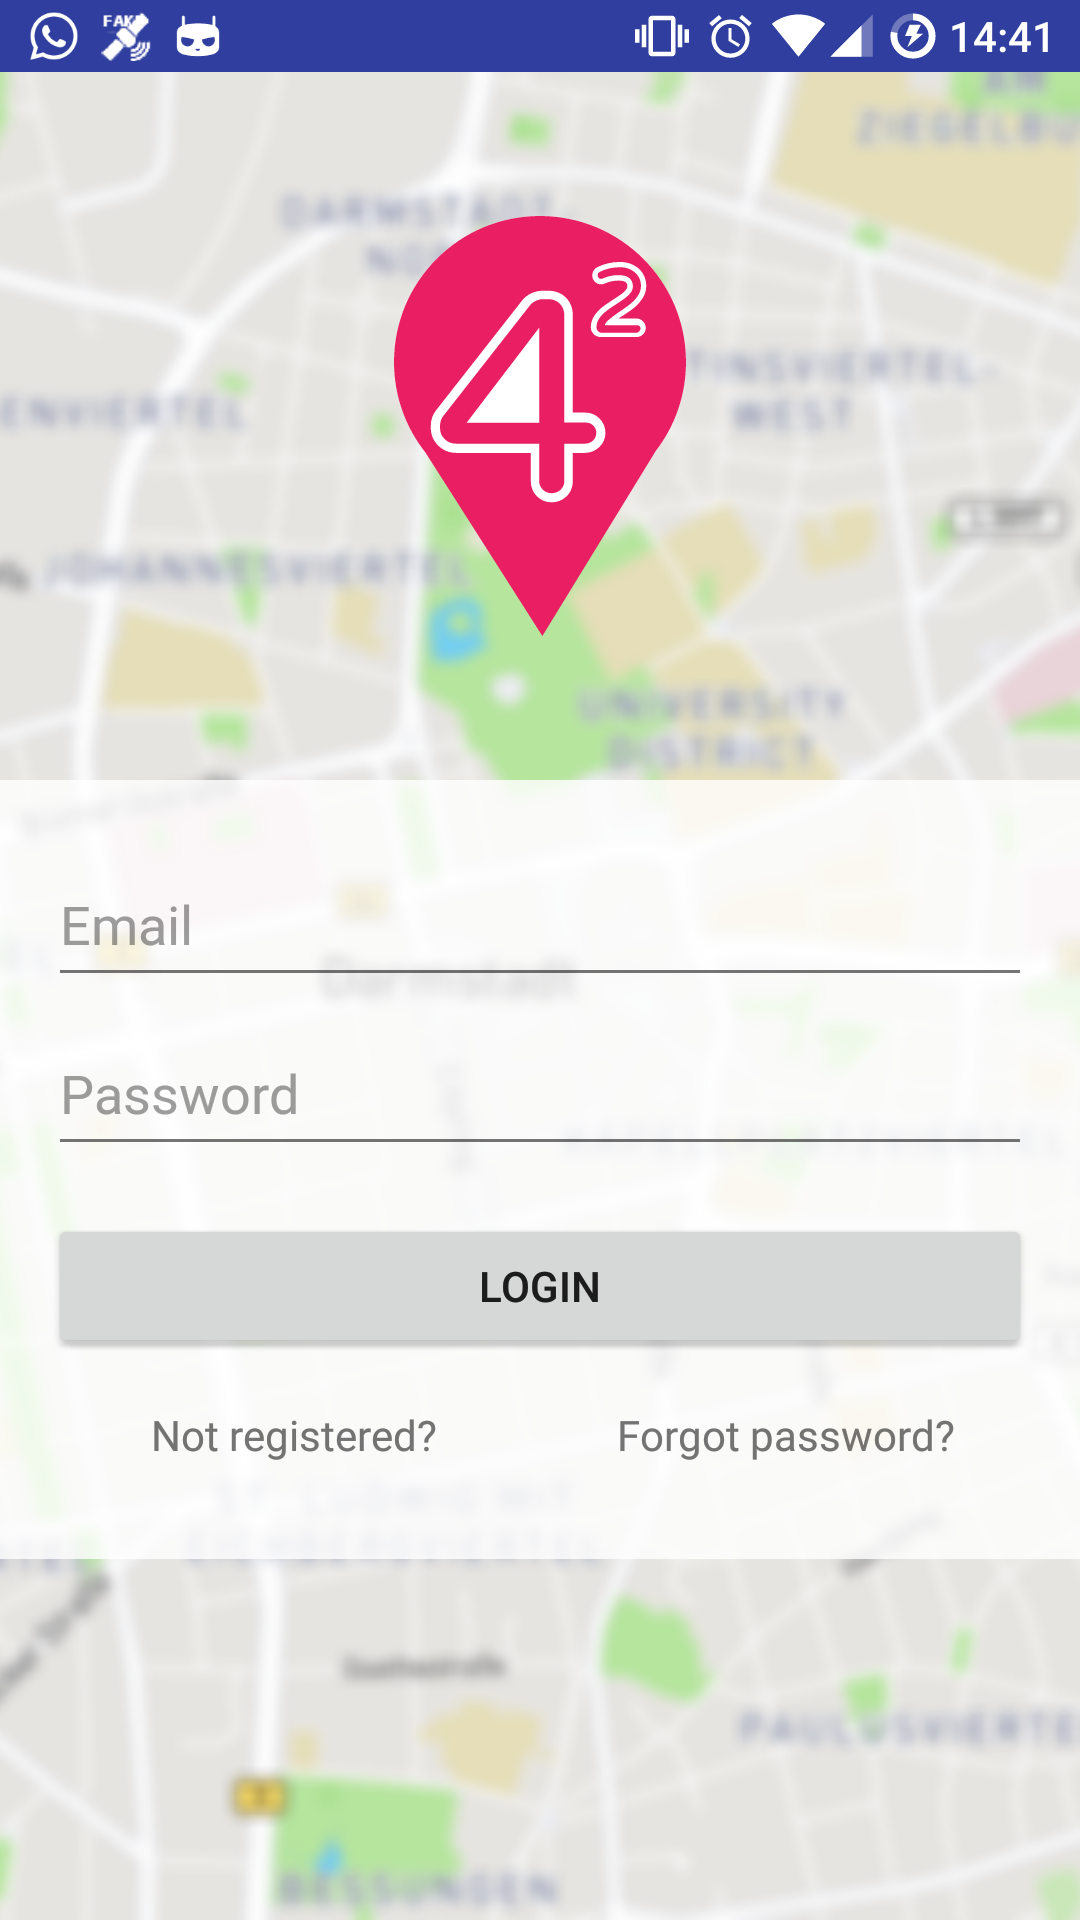
\includegraphics[width=.8\linewidth]{./res/login.png}
  \captionof{figure}{Login View}
  \label{fig:login_view}
\end{minipage}%
\begin{minipage}{.3\textwidth}
  \centering
  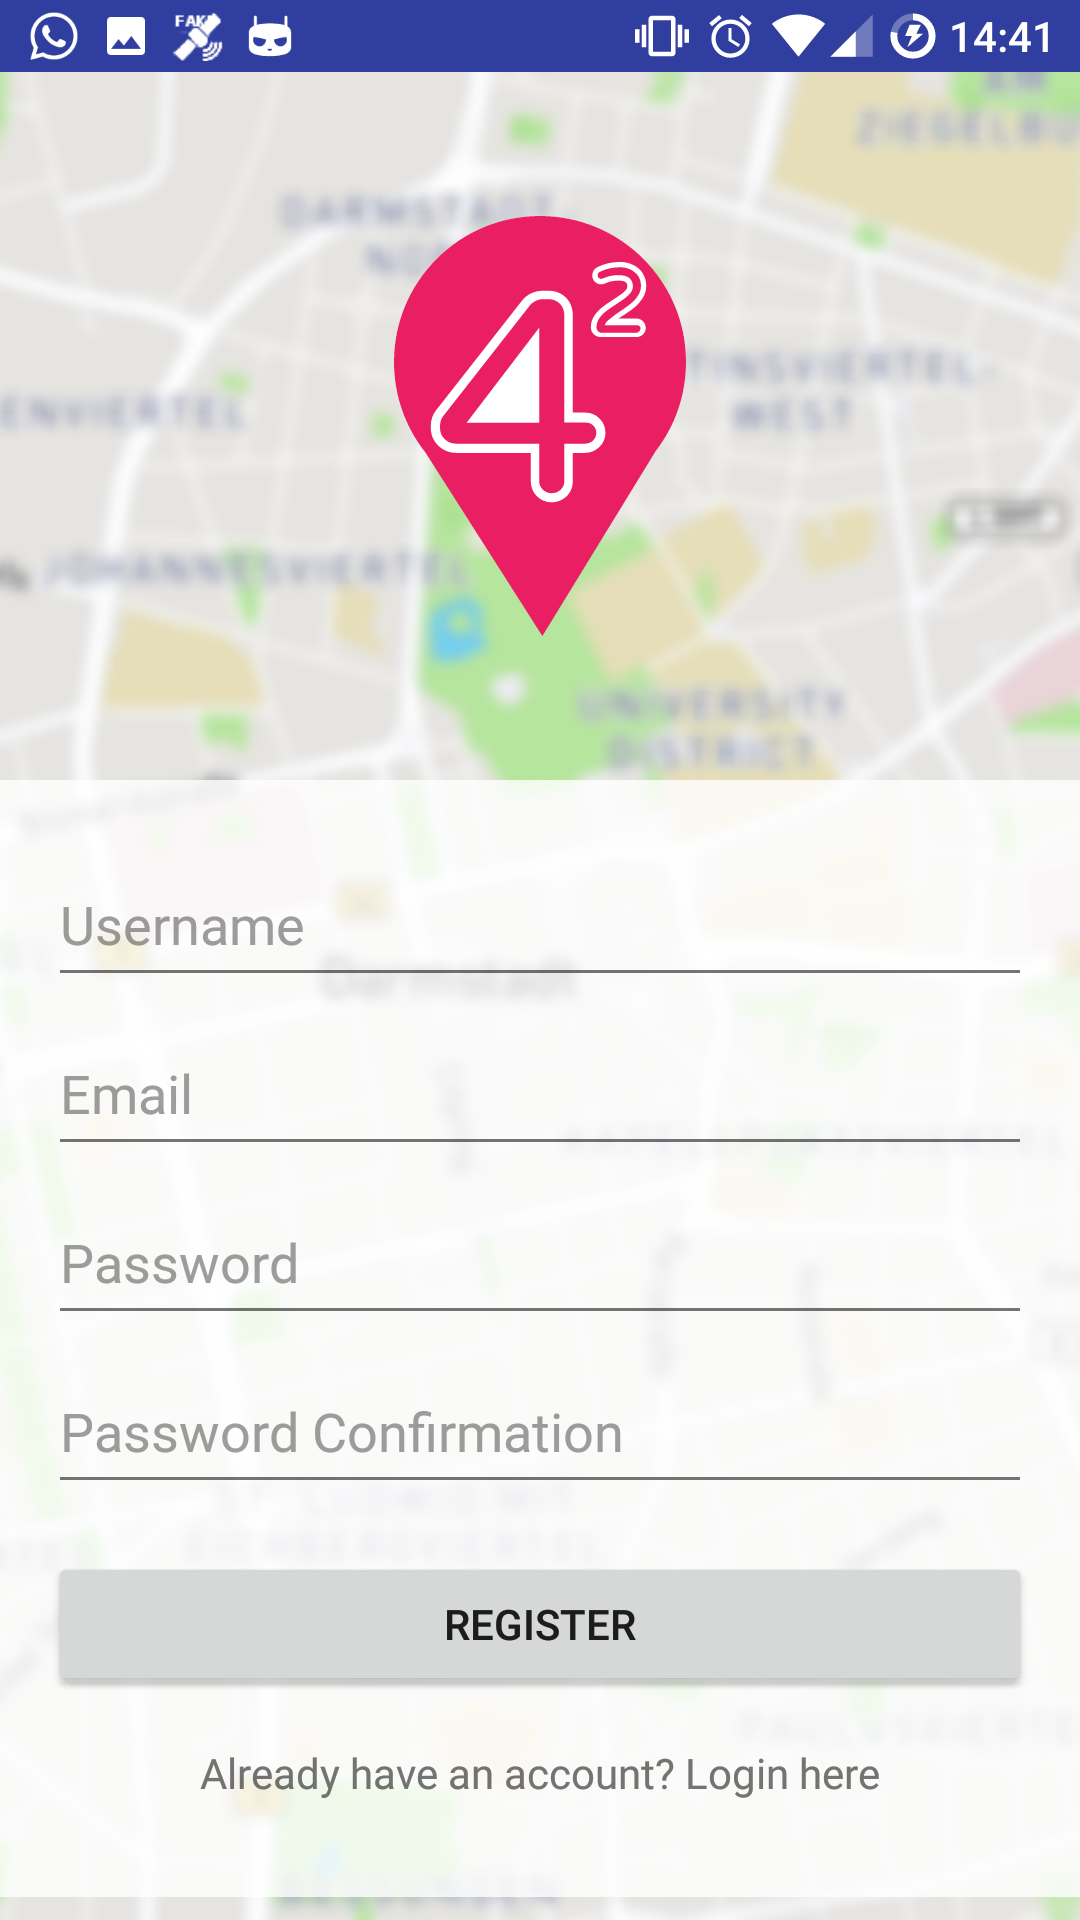
\includegraphics[width=.8\linewidth]{./res/register.png}
  \captionof{figure}{Register View}
  \label{fig:register_view}
\end{minipage}
\begin{minipage}{.3\textwidth}
  \centering
  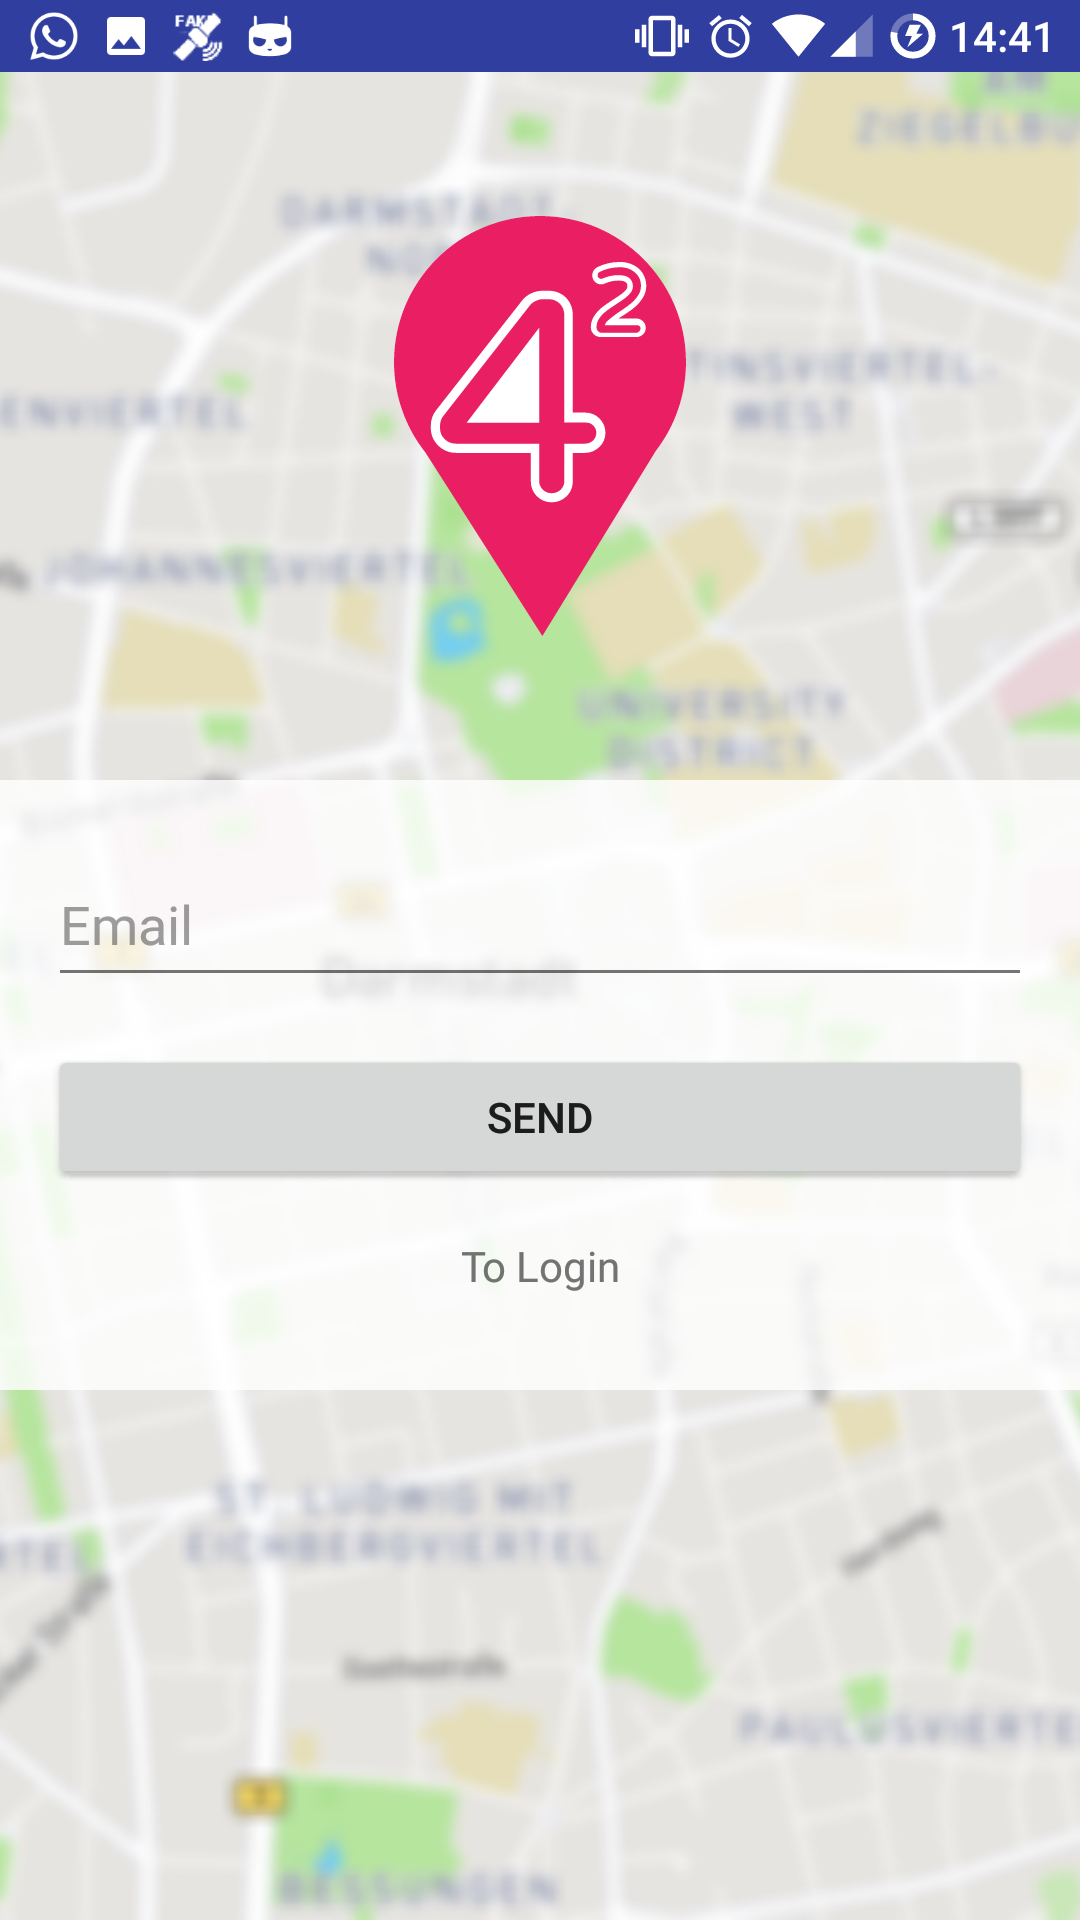
\includegraphics[width=.8\linewidth]{./res/forgotPW.png}
  \captionof{figure}{Forgot PW View}
  \label{fig:forgot_pw_view}
\end{minipage}%
\end{figure}

% Login View
When the user starts our app for the first time, he enters the login view. This view is shown in \autoref{fig:login_view}. If the user enters his login credentials correctly, he is forwarded to the map view shown in \autoref{fig:map_view}. During the first start of our app, the user also has to accept the permissions mentioned in \autoref{sec:system_requirements}. Wrong credentials provided by the user lead to red warnings indicating the problem. The login credentials are stored to improve the user experience by not asking for them every time.

% Register View
If the user has no account to log in, he can create a new one. To do this he has to click on the ``Not registered?'' button. A click on this button directs the user to the register view shown in \autoref{fig:register_view}. The username as well as the mail address have to be unique. With this restriction we can ensure that there is only one account per mail address. We ensure that the password is free of typos by asking for the password two times. Only if the password is entered correctly twice, an account is created. A toast indicates a successful registration. After a successful registration, the user is redirected to the login view and a confirmation mail is sent to the given mail address. The login only works if the mail address is verified. To confirm the account a the link in the email has to be clicked. The smartphone offers the possibility to open the link via a browser or the app ``Sechzehn''. If the link is opened with ``Sechzehn'' the account will be activated and the login screen is shown again.

% Forgot PW View
We also provide the option to reset the account password if necessary (e.g. due to memory loss).
The user can enter the \textit{Forgot PW View} shown in \autoref{fig:forgot_pw_view} by clicking the ``Forgot password?'' button. The user now can enter the email address and click the send button. A password reset request will be sent to that email address. The link in the email could be opened with ``Sechzehn'' or with any browser. If the link in the email is opened with ``Sechzehn'' a screen is opened where you have to insert a new password (two times). By clicking the confirm button the passwords are checked and if they are equal the new password is set. The same procedure could be done on a website by opening the link in a browser.

We further assume that the user is logged in. Now he sees a bottom navigation bar with three navigation options: Search, Friends and Profile. The \textit{Search View} shows a map with venues and users, and offers a search for venues. The \textit{Friends View} shows a list with friends, friendship requests and the last messages. The user profile displays all information we have about the user.

\begin{figure}[h]
\centering
\begin{minipage}{.3\textwidth}
  \centering
  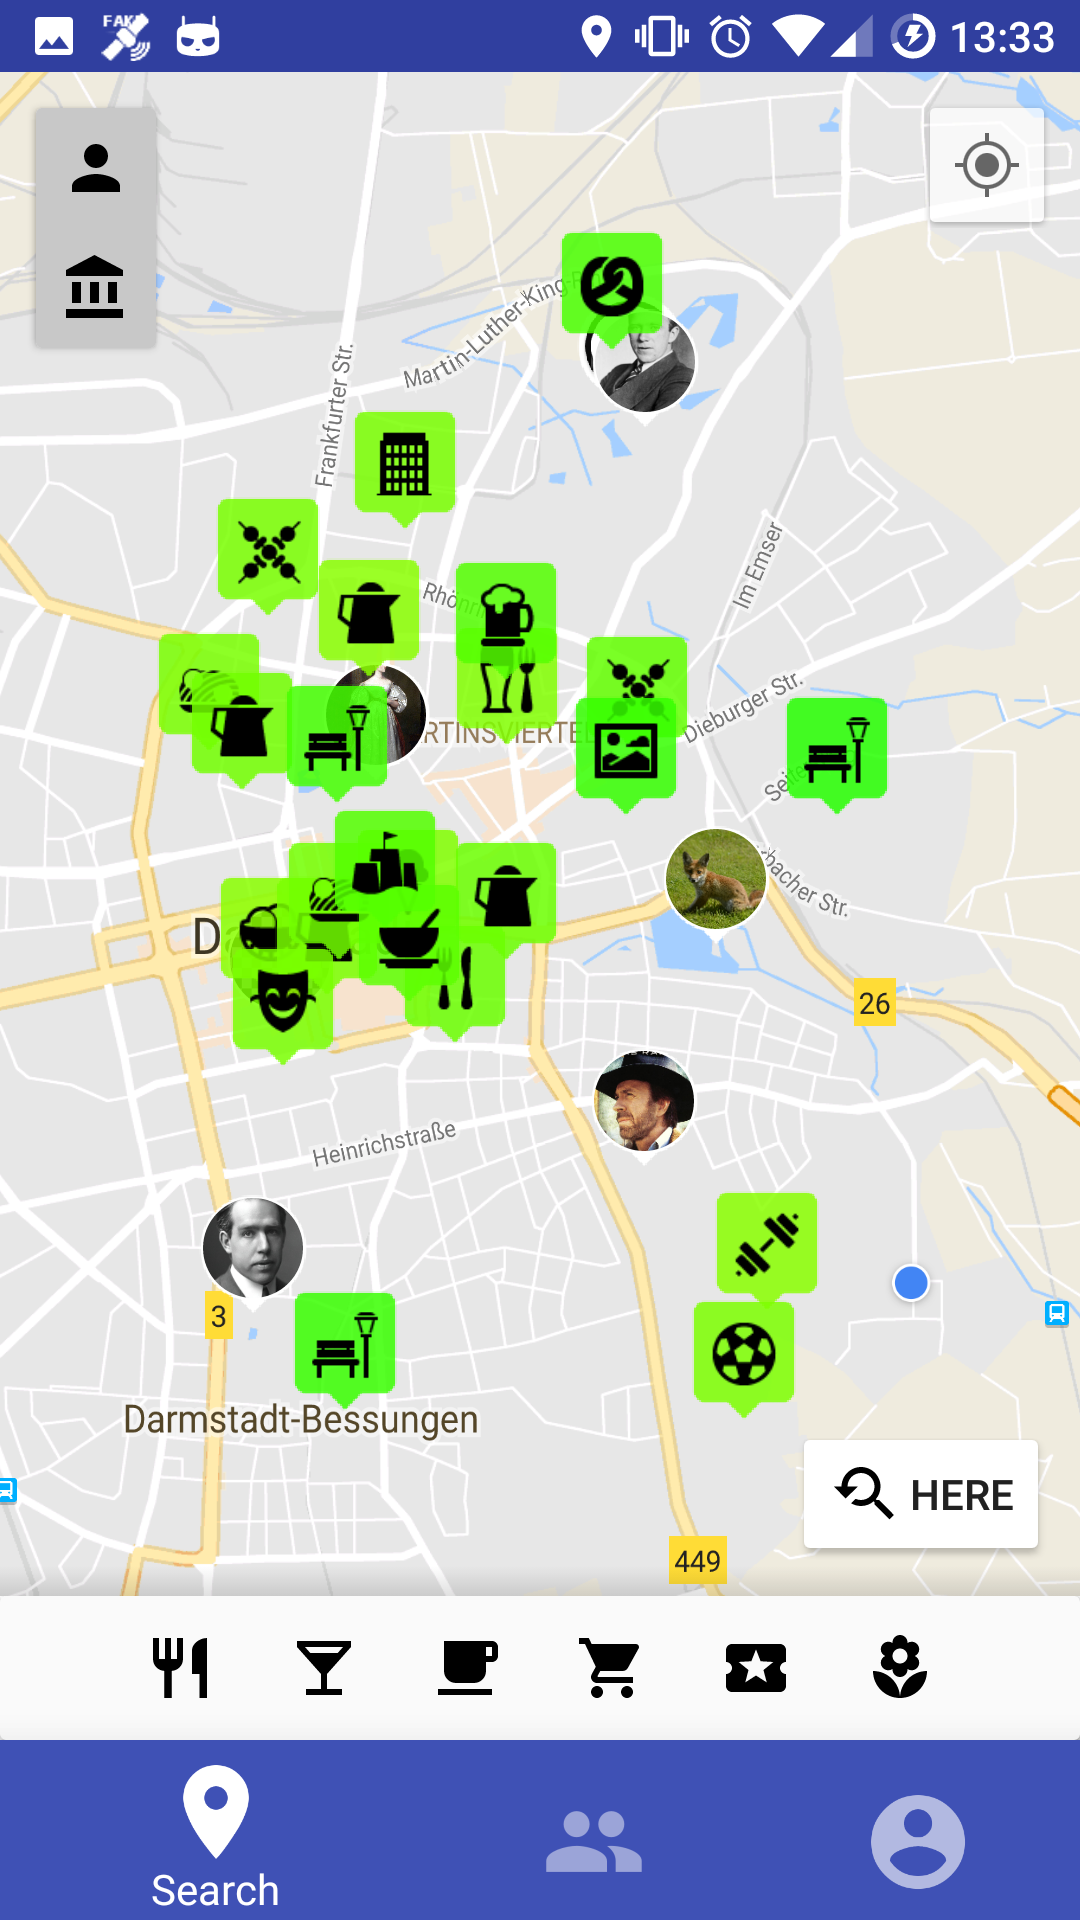
\includegraphics[width=.8\linewidth]{./res/map_user_venues.png}
  \captionof{figure}{Map View}
  \label{fig:map_view}
\end{minipage}%
\begin{minipage}{.3\textwidth}
  \centering
  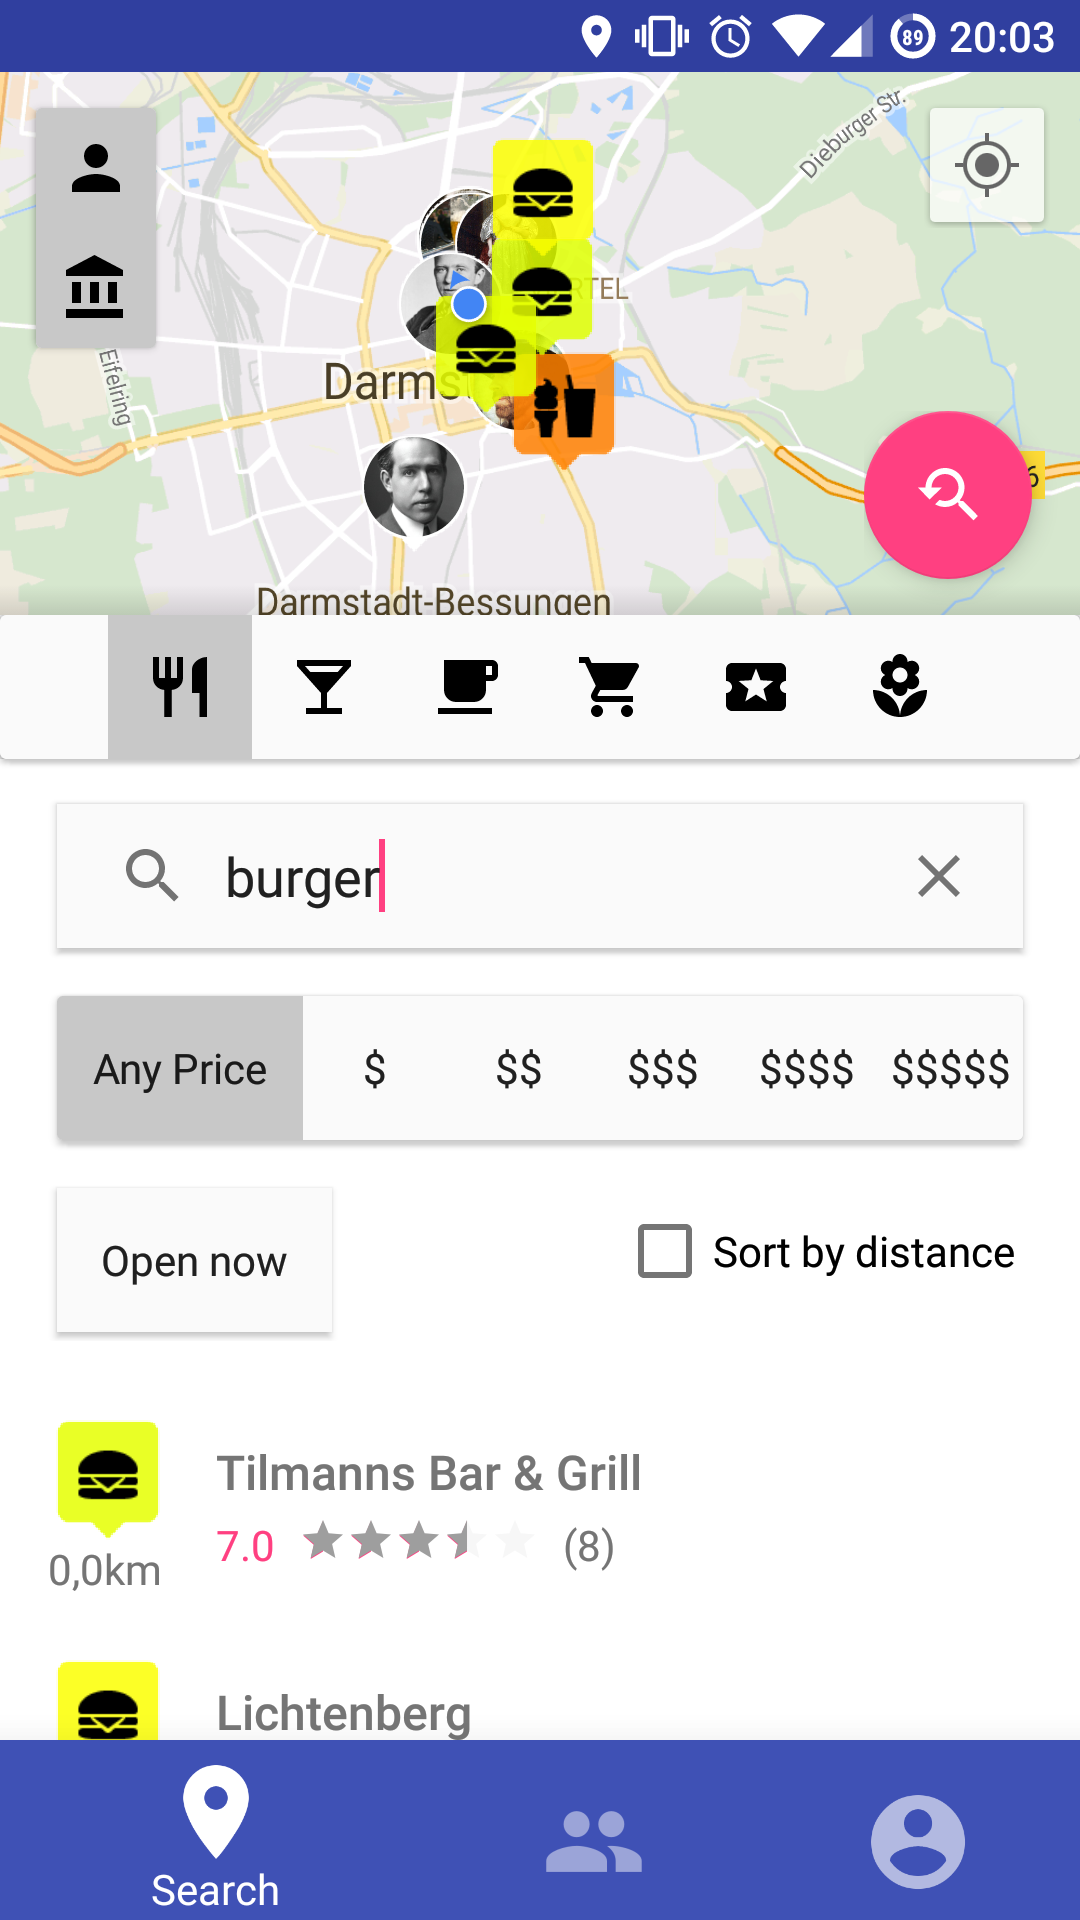
\includegraphics[width=.8\linewidth]{./res/search.png}
  \captionof{figure}{Search View}
  \label{fig:search_view}
\end{minipage}
\begin{minipage}{.3\textwidth}
  \centering
  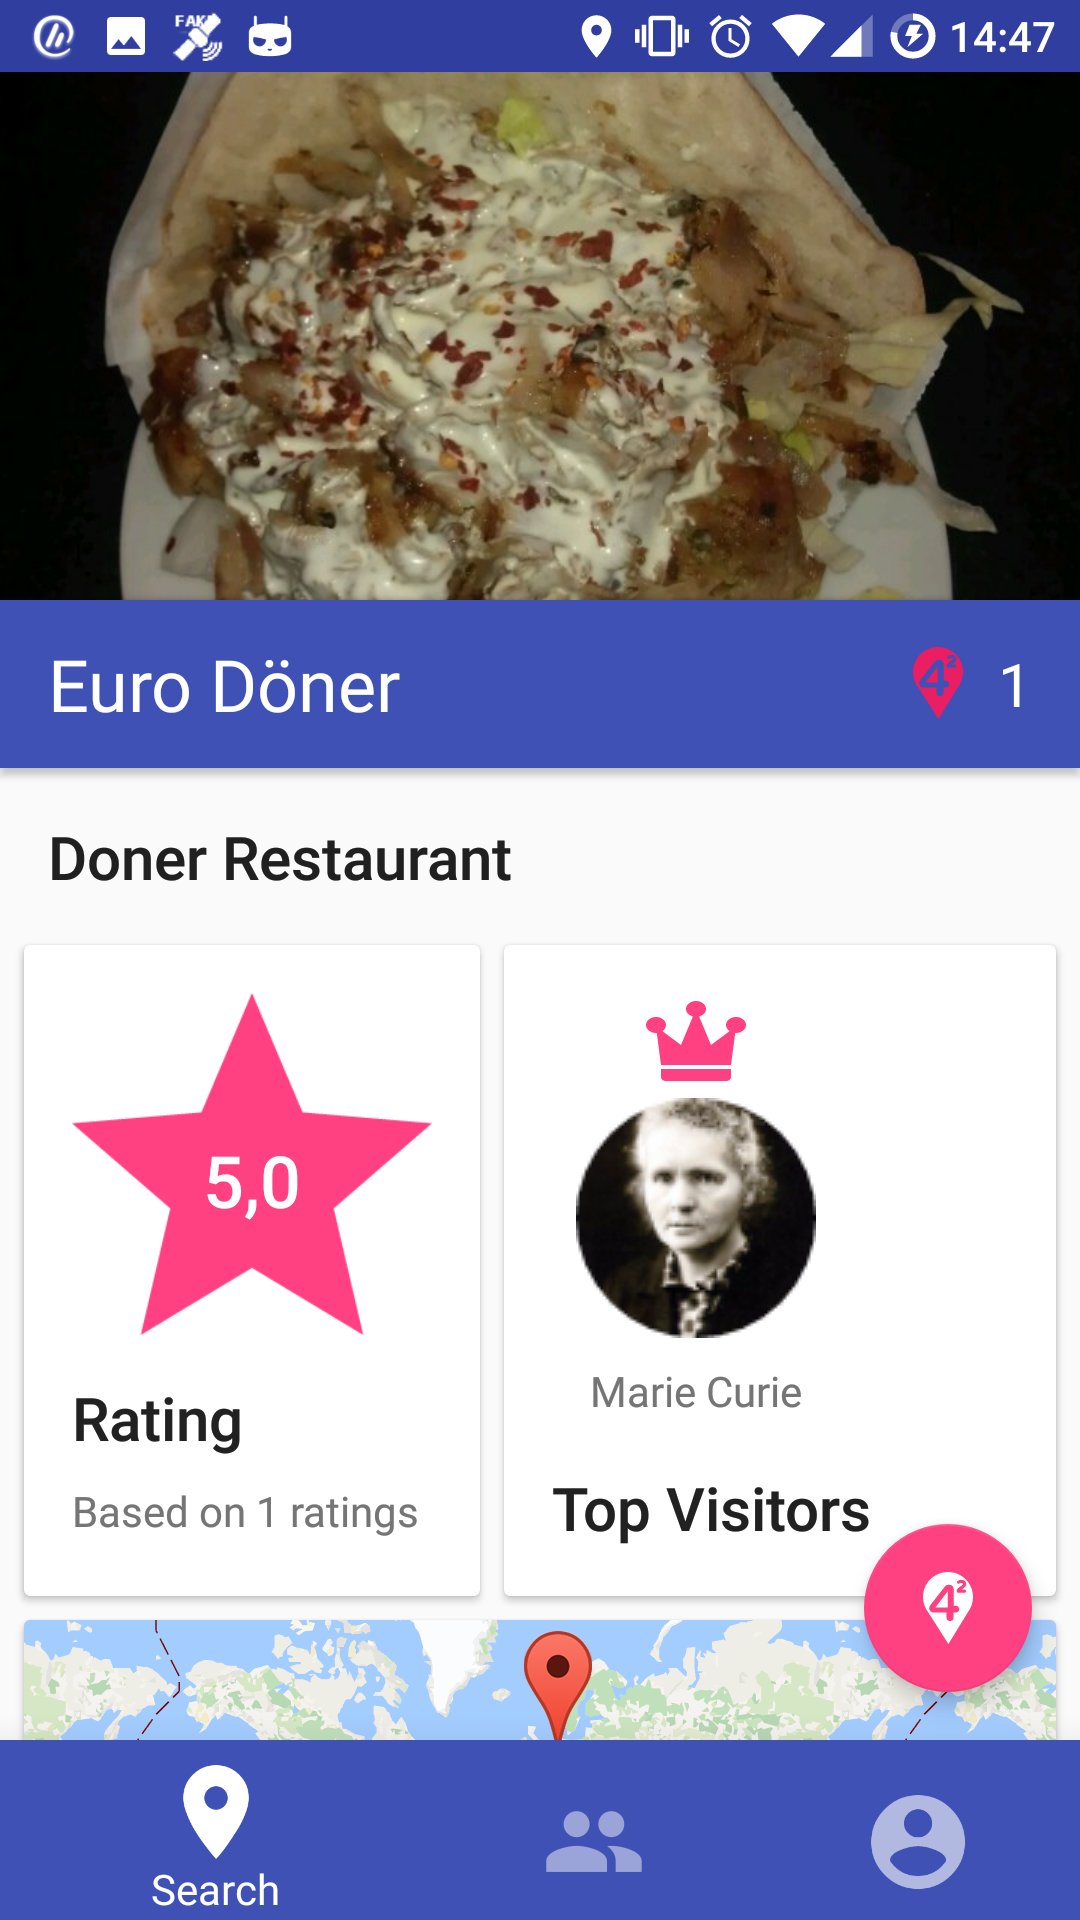
\includegraphics[width=.8\linewidth]{./res/venue.png}
  \captionof{figure}{Venue View}
  \label{fig:venue_view}
\end{minipage}%
\end{figure}

% Map View
The first view appearing after the login, is the map view shown in \autoref{fig:map_view}. Per default it displays users and venues in your surrounding. Two buttons in the top left corner can be used to hide and show venues and users. The six icons right on top of the bottom navigation bar, can be used to trigger fast searches for food, drinks, coffee, shops, arts, and outdoor activities. If the map is moved around the search can be re-triggered by tapping on the floating action button appearing in the bottom right corner.
Tapping on a venue opens the venue view while tapping on a user opens the profile of the user. 
By sliding up the quick search bar, the extensive search view shown in \autoref{fig:search_view}.

% Search View
To find the venue of the users interest, we offer a more extensive search. Besides a keyword search, we also offer filtering for a price category and only displaying venues that are open at the moment. The search results are displayed in the map as well as in a list right below the search query. The filtering for categories mentioned in the previous paragraph, also works in this view. The results can be sorted by rating or by distance.

% Venue View
The venue view is shown in \autoref{fig:venue_view}. The venue view summarizes information about a venue provided by the community. This includes an average rating, pictures of the venue and comments that can contain a photo. Furthermore general information about the venue is shown. With general information we mean opening hours, address, and contact details. With a floating action button it is possible to check in into a venue and rate it. Based on those check ins we provide a bit of gamification: the three top visitors of a venue are highlighted to encourage users using the check in function and thereby rate the venue.


\begin{figure}[h]
\centering
\begin{minipage}{.3\textwidth}
  \centering
  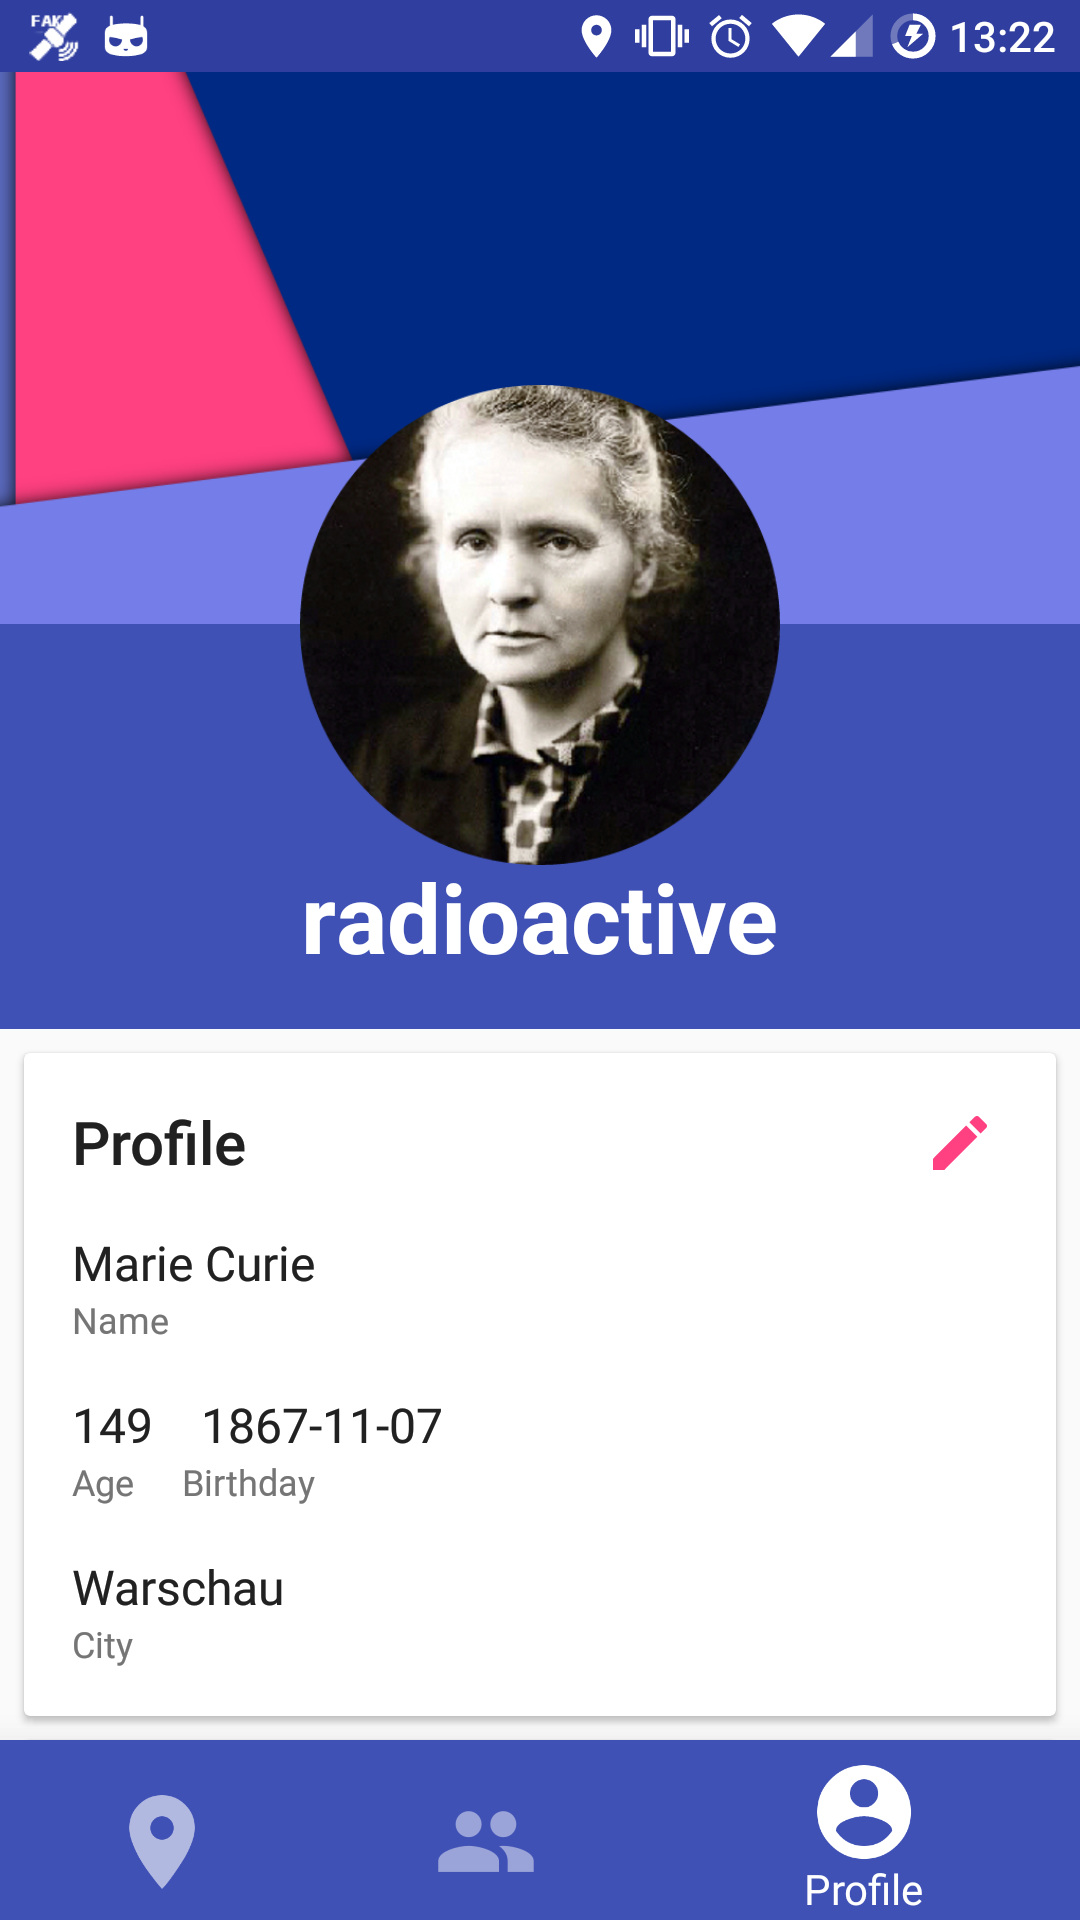
\includegraphics[width=.8\linewidth]{./res/profile.png}
  \captionof{figure}{User Profile}
  \label{fig:user_profile}
\end{minipage}%
\begin{minipage}{.3\textwidth}
  \centering
  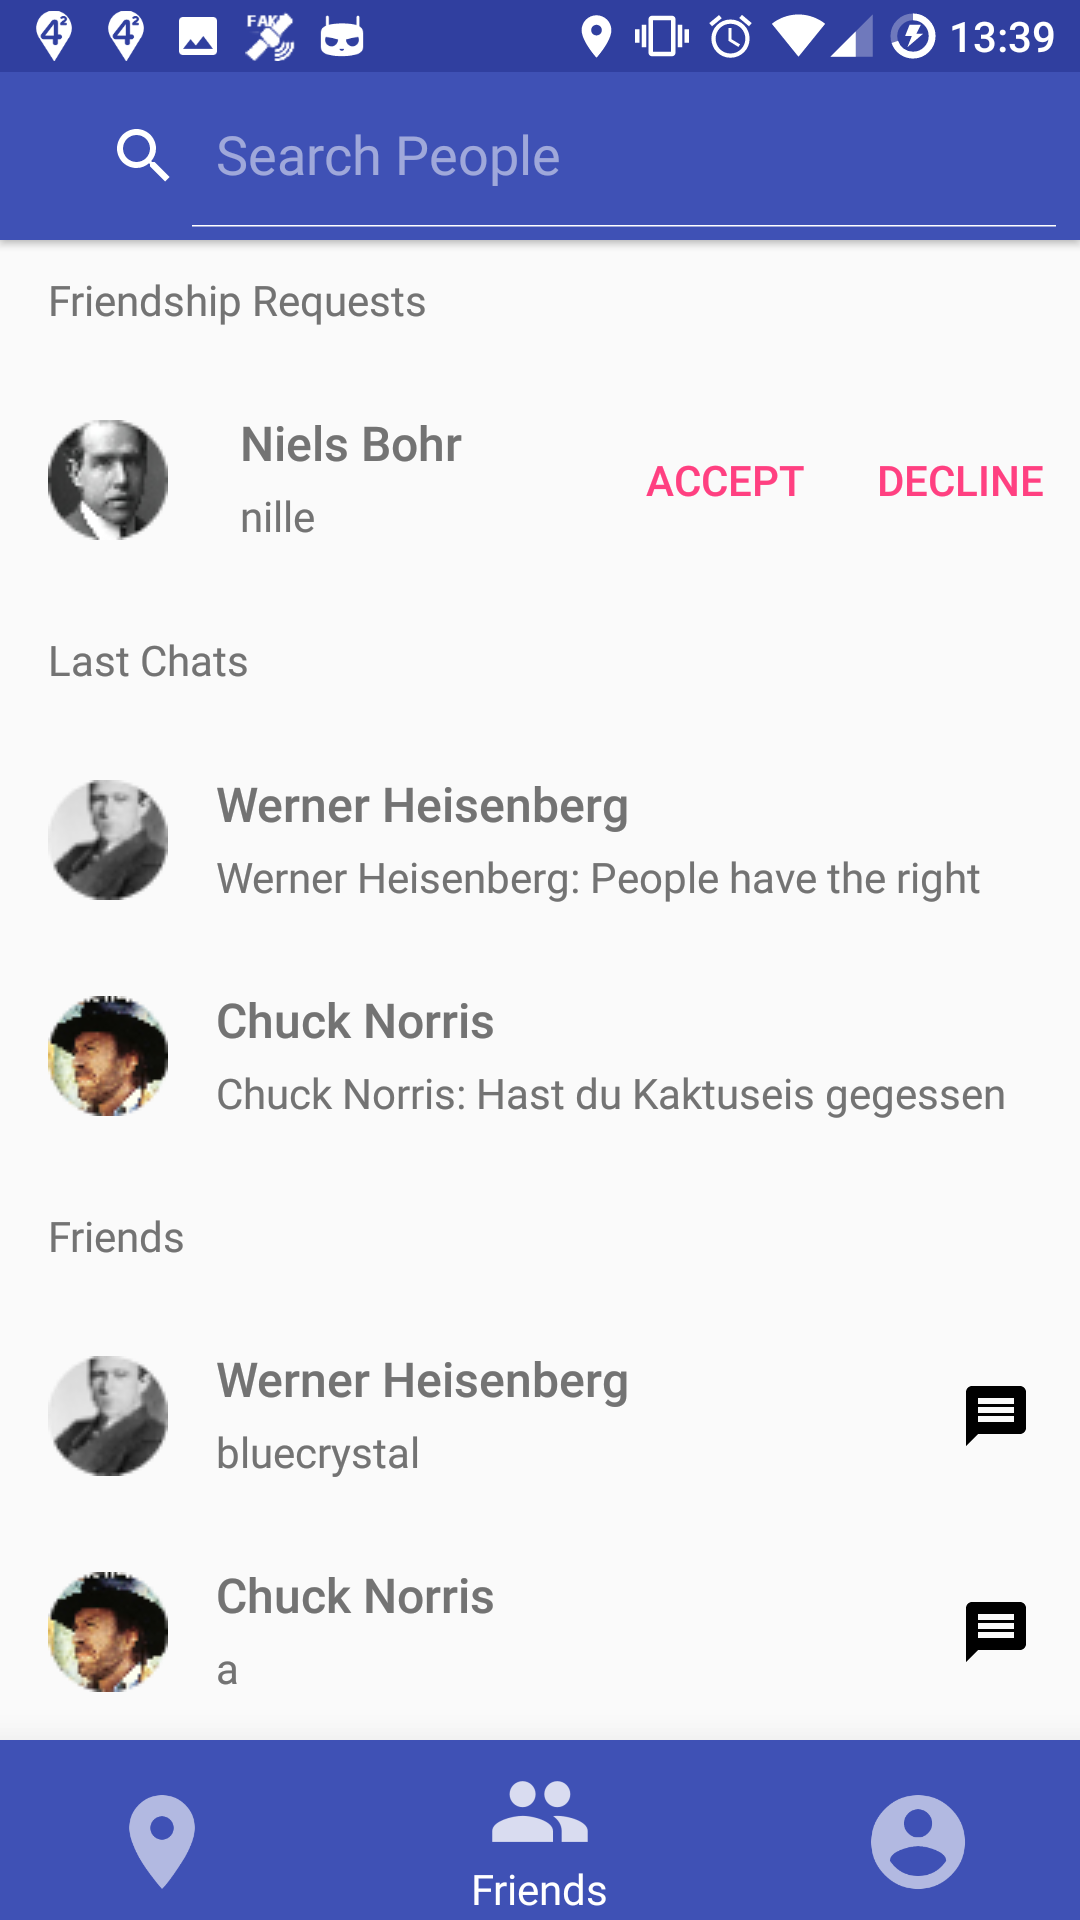
\includegraphics[width=.8\linewidth]{./res/friends.png}
  \captionof{figure}{Friends View}
  \label{fig:friends_view}
\end{minipage}
\begin{minipage}{.3\textwidth}
  \centering
  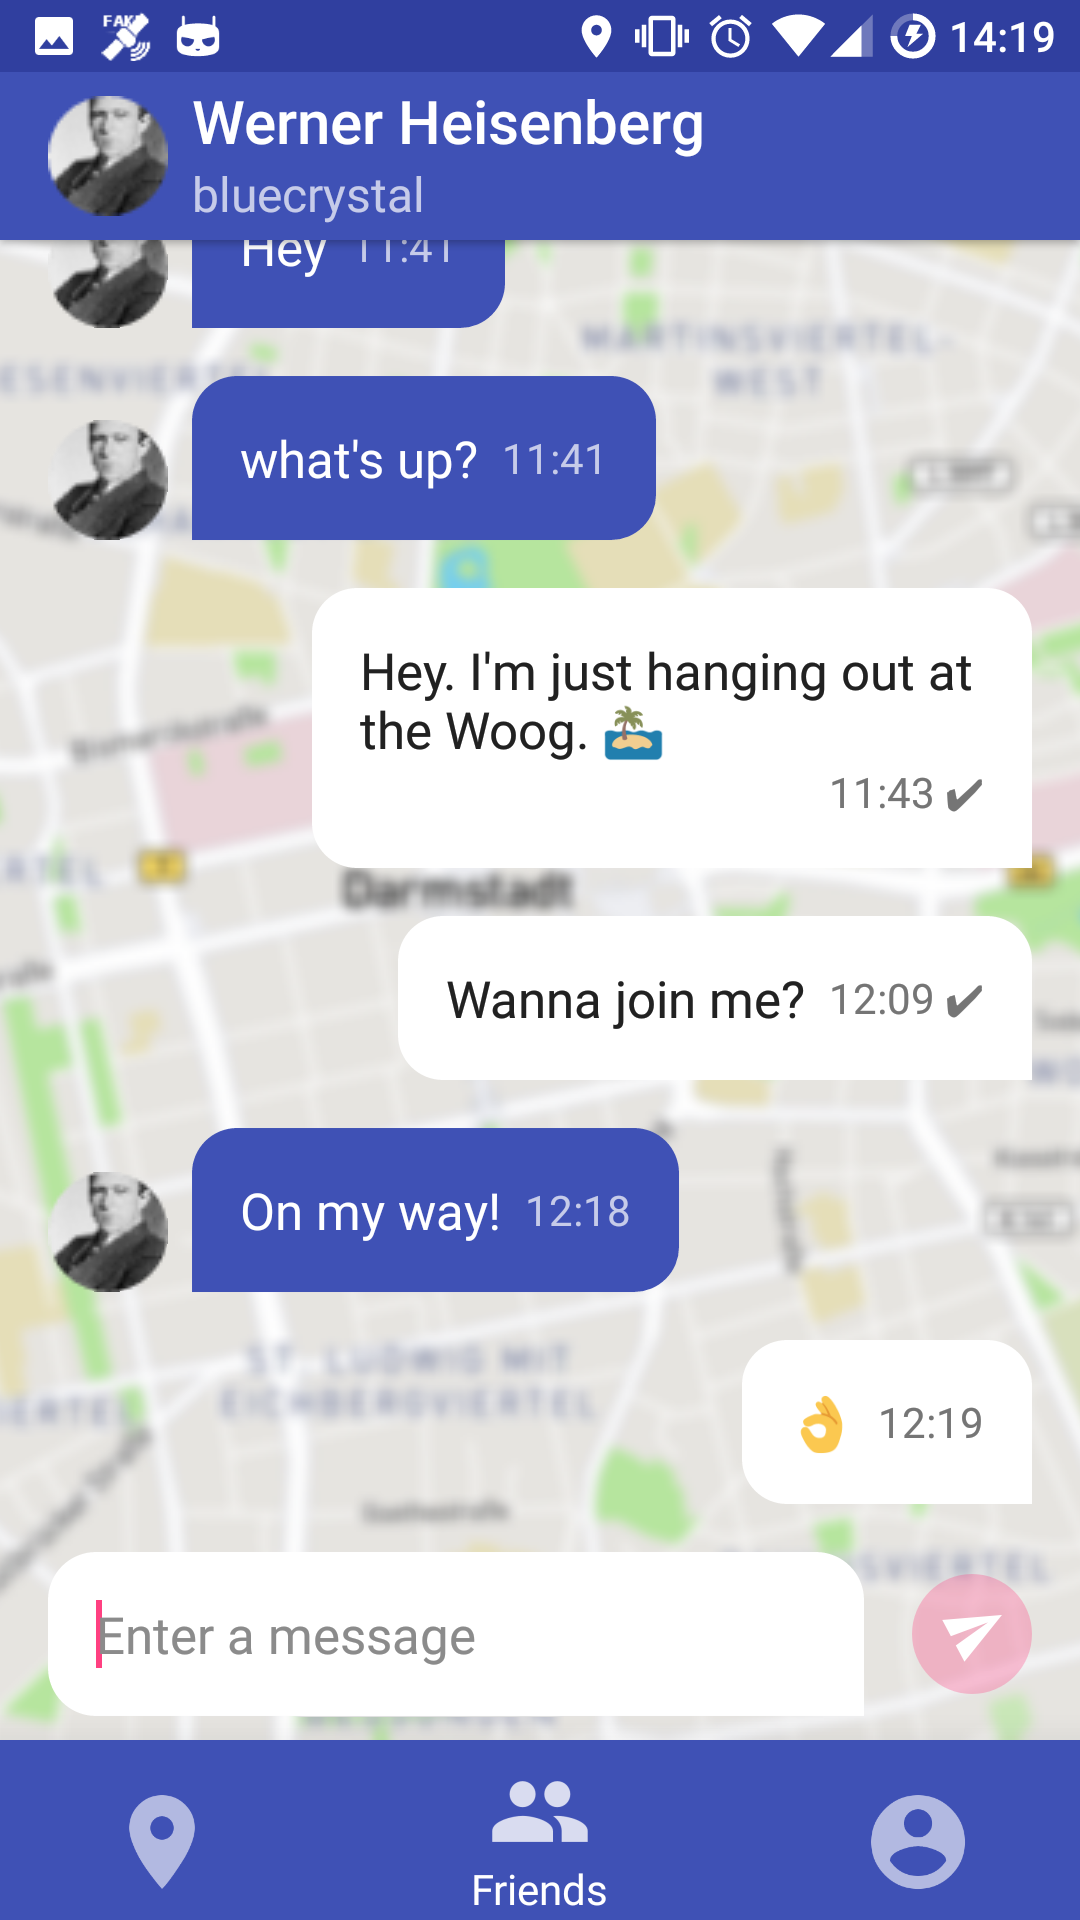
\includegraphics[width=.8\linewidth]{./res/chat.png}
  \captionof{figure}{Live Chat}
  \label{fig:live_chat}
\end{minipage}%
\end{figure}

% User Profile
The profile view is shown in \autoref{fig:user_profile}. The profile picture is on the top of the profile view. By tapping on it, the users photo gallery is opened and he can choose a new profile picture. In the profile section basic information about the user is displayed (respectively real name, age and home town).
This information can be changed by clicking on the small pencil in the top right of the section. In this edit menu you also have the option to toggle the incognito mode described in \autoref{sec:features}. In this view the user can change all of this information. Furthermore this is where the log out option is located. In the bottom of the profile view there are several account settings not described in detail here.

% Friends View
The friends view is shown in \autoref{fig:friends_view}. In the first section open friendship requests are displayed. These requests can be accepted or declined. In the second section the chats are displayed. In the last section the user's friends are shown. By tapping on a friend his profile is shown, by tapping on the message symbol the live chat with the user is invoked. 
All of those sections are only displayed if information in them is available. Without outstanding friendship requests, the section friendship requests is not shown. 
It is tedious to scroll through this growing list. We therefore provided a search bar to filter the list. The search bar is also used to find and add new friends. 

The chat view is shown in \autoref{fig:live_chat}. On the top of the chat view the chat partner is shown.
With a tap on the name of the chat partner, his profile is entered. Checks marks next to the messages indicate that you chat partner has read a message of yours. To make the live chat useful even if the app is not in the foreground, we provide push notifications. This push notifications are displayed for every incoming message. They contain the name of the chat partner and the first few words of the message.


\chapter{Feature List}\label{ch:feature_list}
% ! 1 page !
\begin{itemize}
\item Account:
\begin{itemize}
	\item create an account (registering and confirming email)
\item login (with email and password)
\item password reset if password forgotten (send token and open via app/browser)
\end{itemize}
\item Venue details:
\begin{itemize}
	\item pictures (album with swiping)
\item top visitors (three)
\item contact (address, phone, web)
\item opening hours
\item comments (add new comments (w/ photos)  and rate it) 
\item check in and rate the venue
\end{itemize}
\item Search
\begin{itemize}
	\item list of venues (ordered by rating)
\item map with venues (venues coloured by rating)
\item filterable (by venue category, price category, and opened now)
\end{itemize}
\item Map: 
\begin{itemize}
	\item shows venues on the map (click to view the venue detail)
\item shows user location on the map
\item show friends location (with live updates) 
\end{itemize}
\item User Profile:
\begin{itemize}
	\item show and edit profile (edit name, birthday, city)
\item view/change profile picture
\item logout
\item delete account
\item change email
\item change password (when logged in and old password is known)
\item reset password (with email if password is not known) 
\end{itemize}
\item Friends: 
\begin{itemize}
	\item find friends (by name/username, comments, nearby people (if incognito mode is disabled))
\item friend list (show friends, friendship requests, and link to profile by taping on a user)
\item chat (write messages,see last messages, and become push notification)
\end{itemize}

\end{itemize}
% pls only list the most relevant implemented features

% Bibliography
\begin{thebibliography}{9}
	\bibitem{apiary}
		\textit{Sechzehn API Documentation | Apiary}, 
		Accessed: 2017-08-24, \\
		\url{http://docs.iptk.apiary.io/}
	\bibitem{heroku}
		\textit{Heroku}, 
		Accessed: 2017-08-09, \\
		\url{https://www.heroku.com/}
	\bibitem{cloudinary}
		\textit{Cloudinary Features}, 
		Accessed: 2017-08-09 \\
		\url{http://cloudinary.com/features}
	\bibitem{Node.js}
		\textit{API Reference Documentation}, 
		Accessed: 2017-08-09, \\
		\url{https://nodejs.org/en/docs/}
	\bibitem{adonisjs}
		\textit{AdonisJs at a Glance}, 
		Accessed: 2017-08-09, \\
		\url{https://adonisjs.com/docs/3.2/overview}
	\bibitem{postgresql}
		\textit{PostgreSQL: Documentation}, 
		Accessed: 2017-08-09, \\
		\url{https://www.postgresql.org/docs/}
	\bibitem{jwt}
		\textit{Introduction to JSON Web Tokens}, 
		Accessed: 2017-08-09, \\
		\url{https://jwt.io/introduction/}
	\bibitem{databinding}
		\textit{Data Binding Library}, 
		Accessed: 2017-08-09, \\
		\url{https://developer.android.com/topic/libraries/data-binding/index.html}
	\bibitem{retrofit}
		\textit{Retrofit: A type-safe HTTP client for Android and Java}, 
		Accessed: 2017-08-09, \\	
		\url{https://square.github.io/retrofit/}
	\bibitem{gson}
		\textit{Google GSON}, 
		Accessed: 2017-08-09, \\
		\url{https://github.com/google/gson}
	\bibitem{chatkit}
		\textit{ChatKit for Android}, 
		Accessed: 2017-08-09, \\
		\url{https://github.com/stfalcon-studio/ChatKit}
\end{thebibliography}
\end{document}